% Created by tikzDevice version 0.12.6 on 2024-11-10 11:15:48
% !TEX encoding = UTF-8 Unicode
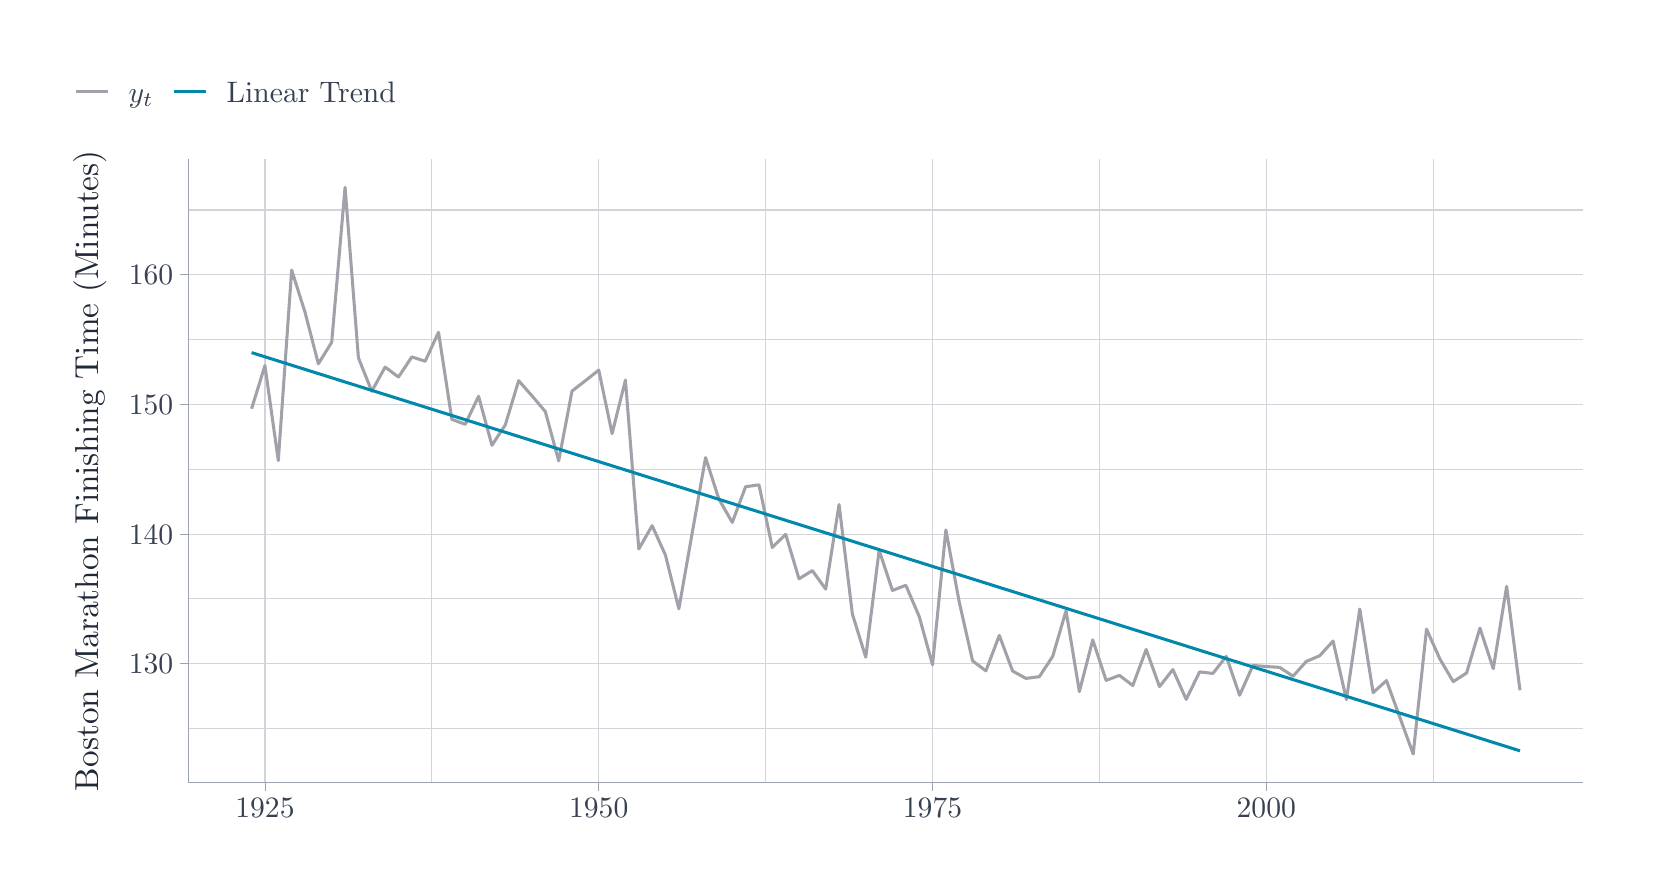
\begin{tikzpicture}[x=1pt,y=1pt]
\definecolor{fillColor}{RGB}{255,255,255}
\path[use as bounding box,fill=fillColor] (0,0) rectangle (578.16,303.53);
\begin{scope}
\path[clip] (  0.00,  0.00) rectangle (578.16,303.53);
\definecolor{drawColor}{RGB}{255,255,255}

\path[draw=drawColor,line width= 0.6pt,line join=round,line cap=round,fill=fillColor] (  0.00,  0.00) rectangle (578.16,303.53);
\end{scope}
\begin{scope}
\path[clip] ( 58.00, 30.82) rectangle (562.16,256.08);
\definecolor{drawColor}{RGB}{255,255,255}
\definecolor{fillColor}{RGB}{255,255,255}

\path[draw=drawColor,line width= 0.6pt,line join=round,line cap=round,fill=fillColor] ( 58.00, 30.82) rectangle (562.16,256.08);
\definecolor{drawColor}{RGB}{209,213,219}

\path[draw=drawColor,line width= 0.4pt,line join=round] ( 58.00, 50.27) --
	(562.16, 50.27);

\path[draw=drawColor,line width= 0.4pt,line join=round] ( 58.00, 97.12) --
	(562.16, 97.12);

\path[draw=drawColor,line width= 0.4pt,line join=round] ( 58.00,143.96) --
	(562.16,143.96);

\path[draw=drawColor,line width= 0.4pt,line join=round] ( 58.00,190.80) --
	(562.16,190.80);

\path[draw=drawColor,line width= 0.4pt,line join=round] ( 58.00,237.64) --
	(562.16,237.64);

\path[draw=drawColor,line width= 0.4pt,line join=round] (146.05, 30.82) --
	(146.05,256.08);

\path[draw=drawColor,line width= 0.4pt,line join=round] (266.66, 30.82) --
	(266.66,256.08);

\path[draw=drawColor,line width= 0.4pt,line join=round] (387.27, 30.82) --
	(387.27,256.08);

\path[draw=drawColor,line width= 0.4pt,line join=round] (507.88, 30.82) --
	(507.88,256.08);

\path[draw=drawColor,line width= 0.4pt,line join=round] ( 58.00, 73.70) --
	(562.16, 73.70);

\path[draw=drawColor,line width= 0.4pt,line join=round] ( 58.00,120.54) --
	(562.16,120.54);

\path[draw=drawColor,line width= 0.4pt,line join=round] ( 58.00,167.38) --
	(562.16,167.38);

\path[draw=drawColor,line width= 0.4pt,line join=round] ( 58.00,214.22) --
	(562.16,214.22);

\path[draw=drawColor,line width= 0.4pt,line join=round] ( 85.74, 30.82) --
	( 85.74,256.08);

\path[draw=drawColor,line width= 0.4pt,line join=round] (206.35, 30.82) --
	(206.35,256.08);

\path[draw=drawColor,line width= 0.4pt,line join=round] (326.97, 30.82) --
	(326.97,256.08);

\path[draw=drawColor,line width= 0.4pt,line join=round] (447.58, 30.82) --
	(447.58,256.08);
\definecolor{drawColor}{RGB}{161,161,170}

\path[draw=drawColor,line width= 1.1pt,line join=round] ( 80.91,165.82) --
	( 85.74,181.43) --
	( 90.56,147.08) --
	( 95.39,215.94) --
	(100.21,200.72) --
	(105.04,182.06) --
	(109.86,189.86) --
	(114.69,245.84) --
	(119.51,184.24) --
	(124.34,172.14) --
	(129.16,180.89) --
	(133.98,177.30) --
	(138.81,184.56) --
	(143.63,182.99) --
	(148.46,193.46) --
	(153.28,161.99) --
	(158.11,160.20) --
	(162.93,170.35) --
	(167.76,152.62) --
	(172.58,159.96) --
	(177.41,175.97) --
	(182.23,170.50) --
	(187.05,164.80) --
	(191.88,147.00) --
	(196.70,172.22) --
	(201.53,175.97) --
	(206.35,179.79) --
	(211.18,156.84) --
	(216.00,176.20) --
	(220.83,115.15) --
	(225.65,123.58) --
	(230.47,112.89) --
	(235.30, 93.53) --
	(240.12,120.93) --
	(244.95,148.17) --
	(249.77,133.19) --
	(254.60,124.75) --
	(259.42,137.64) --
	(264.25,138.34) --
	(269.07,115.70) --
	(273.90,120.46) --
	(278.72,104.38) --
	(283.54,107.34) --
	(288.37,100.63) --
	(293.19,131.23) --
	(298.02, 91.57) --
	(302.84, 76.04) --
	(307.67,114.68) --
	(312.49,100.16) --
	(317.32,102.03) --
	(322.14, 90.79) --
	(326.97, 73.30) --
	(331.79,122.02) --
	(336.61, 96.02) --
	(341.44, 74.71) --
	(346.26, 71.12) --
	(351.09, 83.92) --
	(355.91, 71.04) --
	(360.74, 68.39) --
	(365.56, 69.01) --
	(370.39, 76.35) --
	(375.21, 92.82) --
	(380.03, 63.62) --
	(384.86, 82.28) --
	(389.68, 67.68) --
	(394.51, 69.48) --
	(399.33, 65.81) --
	(404.16, 78.85) --
	(408.98, 65.42) --
	(413.81, 71.59) --
	(418.63, 60.81) --
	(423.46, 70.73) --
	(428.28, 70.18) --
	(433.10, 76.35) --
	(437.93, 62.30) --
	(442.75, 73.07) --
	(447.58, 72.68) --
	(452.40, 72.37) --
	(457.23, 69.17) --
	(462.05, 74.55) --
	(466.88, 76.58) --
	(471.70, 81.89) --
	(476.52, 60.74) --
	(481.35, 93.45) --
	(486.17, 63.23) --
	(491.00, 67.61) --
	(495.82, 54.33) --
	(500.65, 41.06) --
	(505.47, 86.19) --
	(510.30, 75.41) --
	(515.12, 67.22) --
	(519.95, 70.34) --
	(524.77, 86.58) --
	(529.59, 71.90) --
	(534.42,101.64) --
	(539.24, 64.09);
\definecolor{drawColor}{RGB}{1,136,172}

\path[draw=drawColor,line width= 1.1pt,line join=round] ( 80.91,186.11) --
	( 85.74,184.59) --
	( 90.56,183.08) --
	( 95.39,181.56) --
	(100.21,180.05) --
	(105.04,178.53) --
	(109.86,177.02) --
	(114.69,175.50) --
	(119.51,173.99) --
	(124.34,172.47) --
	(129.16,170.96) --
	(133.98,169.45) --
	(138.81,167.93) --
	(143.63,166.42) --
	(148.46,164.90) --
	(153.28,163.39) --
	(158.11,161.87) --
	(162.93,160.36) --
	(167.76,158.84) --
	(172.58,157.33) --
	(177.41,155.82) --
	(182.23,154.30) --
	(187.05,152.79) --
	(191.88,151.27) --
	(196.70,149.76) --
	(201.53,148.24) --
	(206.35,146.73) --
	(211.18,145.21) --
	(216.00,143.70) --
	(220.83,142.18) --
	(225.65,140.67) --
	(230.47,139.16) --
	(235.30,137.64) --
	(240.12,136.13) --
	(244.95,134.61) --
	(249.77,133.10) --
	(254.60,131.58) --
	(259.42,130.07) --
	(264.25,128.55) --
	(269.07,127.04) --
	(273.90,125.52) --
	(278.72,124.01) --
	(283.54,122.50) --
	(288.37,120.98) --
	(293.19,119.47) --
	(298.02,117.95) --
	(302.84,116.44) --
	(307.67,114.92) --
	(312.49,113.41) --
	(317.32,111.89) --
	(322.14,110.38) --
	(326.97,108.86) --
	(331.79,107.35) --
	(336.61,105.84) --
	(341.44,104.32) --
	(346.26,102.81) --
	(351.09,101.29) --
	(355.91, 99.78) --
	(360.74, 98.26) --
	(365.56, 96.75) --
	(370.39, 95.23) --
	(375.21, 93.72) --
	(380.03, 92.20) --
	(384.86, 90.69) --
	(389.68, 89.18) --
	(394.51, 87.66) --
	(399.33, 86.15) --
	(404.16, 84.63) --
	(408.98, 83.12) --
	(413.81, 81.60) --
	(418.63, 80.09) --
	(423.46, 78.57) --
	(428.28, 77.06) --
	(433.10, 75.54) --
	(437.93, 74.03) --
	(442.75, 72.52) --
	(447.58, 71.00) --
	(452.40, 69.49) --
	(457.23, 67.97) --
	(462.05, 66.46) --
	(466.88, 64.94) --
	(471.70, 63.43) --
	(476.52, 61.91) --
	(481.35, 60.40) --
	(486.17, 58.88) --
	(491.00, 57.37) --
	(495.82, 55.86) --
	(500.65, 54.34) --
	(505.47, 52.83) --
	(510.30, 51.31) --
	(515.12, 49.80) --
	(519.95, 48.28) --
	(524.77, 46.77) --
	(529.59, 45.25) --
	(534.42, 43.74) --
	(539.24, 42.22);
\end{scope}
\begin{scope}
\path[clip] (  0.00,  0.00) rectangle (578.16,303.53);
\definecolor{drawColor}{RGB}{156,163,175}

\path[draw=drawColor,line width= 0.3pt,line join=round] ( 58.00, 30.82) --
	( 58.00,256.08);
\end{scope}
\begin{scope}
\path[clip] (  0.00,  0.00) rectangle (578.16,303.53);
\definecolor{drawColor}{RGB}{55,65,81}

\node[text=drawColor,anchor=base east,inner sep=0pt, outer sep=0pt, scale=  1.07] at ( 52.60, 70.02) {130};

\node[text=drawColor,anchor=base east,inner sep=0pt, outer sep=0pt, scale=  1.07] at ( 52.60,116.86) {140};

\node[text=drawColor,anchor=base east,inner sep=0pt, outer sep=0pt, scale=  1.07] at ( 52.60,163.71) {150};

\node[text=drawColor,anchor=base east,inner sep=0pt, outer sep=0pt, scale=  1.07] at ( 52.60,210.55) {160};
\end{scope}
\begin{scope}
\path[clip] (  0.00,  0.00) rectangle (578.16,303.53);
\definecolor{drawColor}{RGB}{156,163,175}

\path[draw=drawColor,line width= 0.3pt,line join=round] ( 55.00, 73.70) --
	( 58.00, 73.70);

\path[draw=drawColor,line width= 0.3pt,line join=round] ( 55.00,120.54) --
	( 58.00,120.54);

\path[draw=drawColor,line width= 0.3pt,line join=round] ( 55.00,167.38) --
	( 58.00,167.38);

\path[draw=drawColor,line width= 0.3pt,line join=round] ( 55.00,214.22) --
	( 58.00,214.22);
\end{scope}
\begin{scope}
\path[clip] (  0.00,  0.00) rectangle (578.16,303.53);
\definecolor{drawColor}{RGB}{156,163,175}

\path[draw=drawColor,line width= 0.3pt,line join=round] ( 58.00, 30.82) --
	(562.16, 30.82);
\end{scope}
\begin{scope}
\path[clip] (  0.00,  0.00) rectangle (578.16,303.53);
\definecolor{drawColor}{RGB}{156,163,175}

\path[draw=drawColor,line width= 0.3pt,line join=round] ( 85.74, 27.82) --
	( 85.74, 30.82);

\path[draw=drawColor,line width= 0.3pt,line join=round] (206.35, 27.82) --
	(206.35, 30.82);

\path[draw=drawColor,line width= 0.3pt,line join=round] (326.97, 27.82) --
	(326.97, 30.82);

\path[draw=drawColor,line width= 0.3pt,line join=round] (447.58, 27.82) --
	(447.58, 30.82);
\end{scope}
\begin{scope}
\path[clip] (  0.00,  0.00) rectangle (578.16,303.53);
\definecolor{drawColor}{RGB}{55,65,81}

\node[text=drawColor,anchor=base,inner sep=0pt, outer sep=0pt, scale=  1.07] at ( 85.74, 18.07) {1925};

\node[text=drawColor,anchor=base,inner sep=0pt, outer sep=0pt, scale=  1.07] at (206.35, 18.07) {1950};

\node[text=drawColor,anchor=base,inner sep=0pt, outer sep=0pt, scale=  1.07] at (326.97, 18.07) {1975};

\node[text=drawColor,anchor=base,inner sep=0pt, outer sep=0pt, scale=  1.07] at (447.58, 18.07) {2000};
\end{scope}
\begin{scope}
\path[clip] (  0.00,  0.00) rectangle (578.16,303.53);
\definecolor{drawColor}{RGB}{31,41,55}

\node[text=drawColor,rotate= 90.00,anchor=base,inner sep=0pt, outer sep=0pt, scale=  1.20] at ( 25.43,143.45) {Boston Marathon Finishing Time (Minutes)};
\end{scope}
\begin{scope}
\path[clip] (  0.00,  0.00) rectangle (578.16,303.53);
\definecolor{drawColor}{RGB}{255,255,255}
\definecolor{fillColor}{RGB}{255,255,255}

\path[draw=drawColor,line width= 0.6pt,line join=round,line cap=round,fill=fillColor] ( 16.00,268.08) rectangle (132.85,287.53);
\end{scope}
\begin{scope}
\path[clip] (  0.00,  0.00) rectangle (578.16,303.53);
\definecolor{drawColor}{RGB}{255,255,255}
\definecolor{fillColor}{RGB}{255,255,255}

\path[draw=drawColor,line width= 0.6pt,line join=round,line cap=round,fill=fillColor] ( 16.00,273.08) rectangle ( 30.45,287.53);
\end{scope}
\begin{scope}
\path[clip] (  0.00,  0.00) rectangle (578.16,303.53);
\definecolor{drawColor}{RGB}{161,161,170}

\path[draw=drawColor,line width= 1.1pt,line join=round] ( 17.45,280.31) -- ( 29.01,280.31);
\end{scope}
\begin{scope}
\path[clip] (  0.00,  0.00) rectangle (578.16,303.53);
\definecolor{drawColor}{RGB}{255,255,255}
\definecolor{fillColor}{RGB}{255,255,255}

\path[draw=drawColor,line width= 0.6pt,line join=round,line cap=round,fill=fillColor] ( 51.44,273.08) rectangle ( 65.90,287.53);
\end{scope}
\begin{scope}
\path[clip] (  0.00,  0.00) rectangle (578.16,303.53);
\definecolor{drawColor}{RGB}{1,136,172}

\path[draw=drawColor,line width= 1.1pt,line join=round] ( 52.89,280.31) -- ( 64.45,280.31);
\end{scope}
\begin{scope}
\path[clip] (  0.00,  0.00) rectangle (578.16,303.53);
\definecolor{drawColor}{RGB}{55,65,81}

\node[text=drawColor,anchor=base west,inner sep=0pt, outer sep=0pt, scale=  1.07] at ( 36.45,276.63) {$y_t$};
\end{scope}
\begin{scope}
\path[clip] (  0.00,  0.00) rectangle (578.16,303.53);
\definecolor{drawColor}{RGB}{55,65,81}

\node[text=drawColor,anchor=base west,inner sep=0pt, outer sep=0pt, scale=  1.07] at ( 71.90,276.63) {Linear Trend};
\end{scope}
\end{tikzpicture}
